
\subsection{Performance}
\label{sec:results:performance}

The single allocation benchmark results is presented in Figure~\ref{fig:allocation_performance}. It is observed that initializing the memory after allocating have negligible effect on performance when performed right after the allocation request. Performing the absolute worst-case allocation, when only a larger block exists, is shown to be slower in all cases than when a suitable block exists. This is expected since more work is done in this case than when a suitable block exists. Furthermore, the optimized version is on par with the performance of the reference version, while the general version is slower than the other two versions. 

\begin{figure}[H]
    \centering
    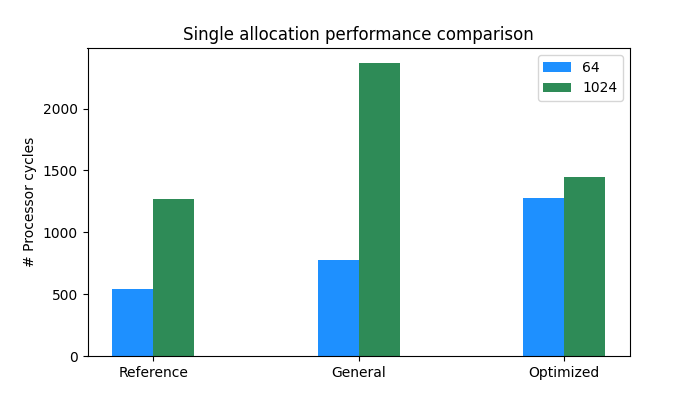
\includegraphics[width=0.90\textwidth]{figures/allocation_performance.png}
    \caption{Allocation performance when allocating 64 bytes on the different versions of the allocator when there is (1) a 64 byte block and (2) a 1024 byte block present in the allocator.}
    \label{fig:allocation_performance}
\end{figure}

The relative performance results when applying patterns of allocations and frees are shown in Figure~\ref{fig:program_benchmarks}, and absolute values in Table~\ref{table:program_benchmarks}. Results are shown as the mean of 100000 iterations. We can observe that the reference version is about 15\% faster in all programs and that the general and optimized versions are on-par in most programs. There is an overhead of logistically applying the allocations and frees, which is added to all programs. As such, the results include this overhead.

\begin{figure}[H]
    \centering
    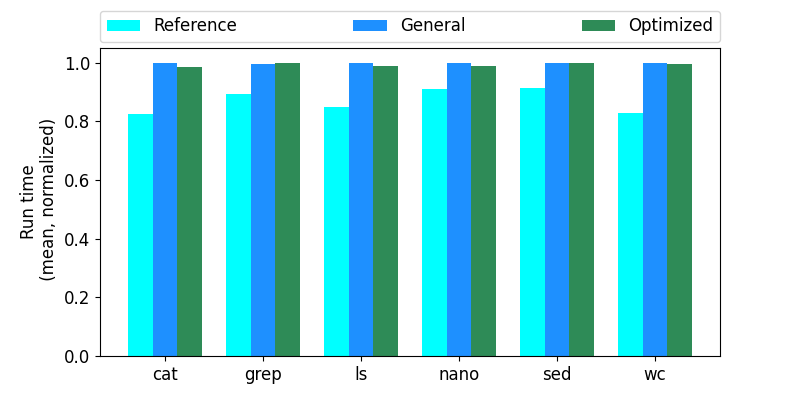
\includegraphics[width=0.90\textwidth]{figures/program_benchmark.png}
    \caption{Scaled run time when applying patterns from different programs The graph is linearly scaled such that the maximum value is 1.0}
    \label{fig:program_benchmarks}
\end{figure}

\begin{table}[H]
    \centering
    \begin{tabular}{lrrrrrr}
    {} & {cat} & {grep} & {ls} & {nano} & {sed} & {wc} \\
    \midrule
    Reference & 601.80 & 5642.16 & 1223.35 & 81184.00 & 9378.62 & 655.73 \\
    General & 729.46 & 6296.89 & 1439.23 & 89139.11 & 10262.90 & 790.35 \\
    Optimized & 718.12 & 6322.36 & 1421.11 & 88042.78 & 10284.13 & 786.14 \\
    \end{tabular}
    \caption{Mean benchmark results when applying patterns from different programs. Results are given in microseconds.}
    \label{table:program_benchmarks}
\end{table}

\subsection{Internal Fragmentation}

The size of the block header for the different versions are: 32 bytes, of which 16 bytes can be used by allocated blocks for the reference version; 32 bytes for the general version; and 0 bytes for the optimized version. 

In the worst case with maximum padding necessary, the reference version will waste up to 57.5\%, general version 69.6\% and the optimized version 29.2\%, if filling the heap with as many allocations as possible of 17 bytes. Looking at the second case where there is no padding necessary for alignment, the reference version will waste up to 50\%, general version 66\% and the optimized version 0\%, if filling the heap with as many allocations as possible of 16 bytes.

To summarize, when filling the heap with as small allocations as possible and considering the size of the block header and any necessary padding due to alignment, the reference version will waste 50\%-57.5\%, general version 66\%-69.6\% and the optimized version 0\%-29.2\%, depending on the amount of padding that is applied. This means that for the optimized version, the single source of internal fragmentation is due to the padding that is applied.

% Worst case for reference is when the blockheader + alignment is maximum.

% Assumptions:
%  - 2MB heap, largest allocation is 256KB, smallest is 16B, alignment is 8B

% Three cases, fill the heap with allocations of same size:
% Case 1 (worst case for reference):
%  - 17B
% Case 2 (no alignment padding, only block header overhead)
%  - 16B

% Case 3 (worst case for optimized version, maximum alignment)
%  - 17B
% Note: Best case for optimized is any multiple of MBS (16B), Case 2 shows this.

% Referencess
% ----------------------------------------------
% Case 1:
%  - [ BlockHeader (16B) ][ Allocation (17B) + Alignment (7B) ]
%  - Waste is: 16 + 7 = 23B
%  - Num blocks: 2MB / 40B = 52428.8 = 52428
%  - Min waste: 52428 * 23 / 2MB = 0.57499122619
% Case 2:
%  - [ BlockHeader (16B) ][ Allocation (16B) ]
%  - Waste is 16B
%  - Num blocks: 2MB / 16B = 65536
%  - Min waste: 65536 * 16 / 2MB = 0.5

% General
% ----------------------------------------------
% Case 1:
%  - [ BlockHeader (32B) ][ Allocation (17B) + Alignment (7B) ]
%  - Waste is: 32 + 7 = 39B
%  - Num blocks: 2MB / 56B = 37449.1607143 = 37449
%  - Min waste: 37449 * 39 / 2MB = 0.69642591476
% Case 2:
%  - [ BlockHeader (32B) ][ Allocation (16B) ]
%  - Waste is 32
%  - Num blocks: 2MB / 48 = 43690
%  - Min waste: 43690 * 32 / 2MB = 0.66665649414

% Optimized
% ----------------------------------------------
% Case 1:
%  - [ BlockHeader (0B) ][ Allocation (17B) + Alignment (7B) ]
%  - Waste is: 7B
%  - Num blocks: 2MB / 24B = 87381.3333333 = 87381
%  - Min waste: 87381 * 7 / 2MB = 0.29166555404
% Case 2:
%  - [ BlockHeader (0B) ][ Allocation (16B) ]
%  - Waste is 0
%  - Internal fragmentation is 0B (0%)













% General
% ----------------------------------------------
% Case 1:
%  - [ BlockHeader (32B) ][ Allocation (17B) + Alignment (7B)]

% Case 2:
%  - MBS = 32
%  - sizeof(BlockHeader) = 32, minimum allocation is 16, which is aligned to MBS
%  - Min alloc is:   [ BlockHeader (32B) ][ Allocation (16B) + Alignment (16B) ]
%  - Waste is: Header + Alignment = 48B
%  - Number of mins: 2MB / 64B = 32768
%  - Min mem waste: 32768 * 48 / 2MB = 0.75
%  - Internal fragmentation is 1572864 (75%)

% Case3:
%  - [ BlockHeader (32B) ][ Allocation (17B) + Alignment (15B) ]
%  - Waste is 32 + 15 = 47B
%  - Number of allocs: 2MB / 64B = 32768
%  - 32768 * 47 / 2MB = 0.734375
%  - Internal fragmentation is 1540096B (73.4%)

% Optimized
% ----------------------------------------------
% Case 1:
%  - 8 allocations
%  - BlockHeaders are 0-byte for allocated objects. Internal fragmentation is only due to alignment.
%  - Internal fragmentation is 0B (0%)

% Case 2:
%  - MBS = 16
%  - Min Alloc is [ BlockHeader (0B) ][ Allocation (16B) + Alignment (0B) ]
%  - In this case there is no internal fragmentation
%  - Internal fragmentaiton is 0B (0%).


% Case 3:
%  - Worst allocation for the optimized version is [ Allocation (17B) + Alignment (15B) ] = 32B
%  - 2MB / 32B = 65536
%  - 65536 * 15 / 2MB = 0.46875
%  - Internal fragmentation is 983040B (46.9%)

% Conclusions
% ----------------------------------------------
% Due to interanl fragmentation, the version will waste at most:
% Reference: 75%
% Optimized: 46.9%

%%% Local Variables:
%%% mode: latex
%%% TeX-master: "main"
%%% End:
